\documentclass[]{article}
\usepackage{graphicx}
\usepackage{float}
\usepackage[margin=0.5in]{geometry}
%opening
\title{{\textbf{Hypothesis}}}
\author{{\textbf {SEPTEMBER}}}

\begin{document}

\maketitle

\section{{\large Hypothesis}}
{\textbf {Hypothesis}} is a Python library for creating unit tests which are simpler to write and more powerful when run, finding edge cases in your code you wouldn’t have thought to look for. 
Hypothesis lets you write tests which instead look like this: 
\begin{enumerate}
	\item For all data matching some specification. 
	\item Perform some operations on the data.  
	\item Assert something about the result.
\end{enumerate}
It generate arbitrary data matching some input specification and checks that some guarantee holds on the output for the generated input, whatever it is. It also saves examples where problems were found to use them for testing again in the future.
 

\section{{\large Getting Started with Hypothesis}}
The main important feature of hypothesis is using strategies for generating different inputs meeting some input specification.
\begin{figure}[H]
	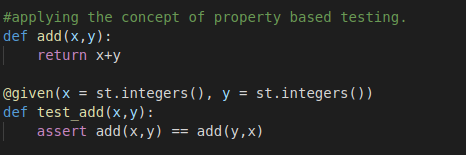
\includegraphics[width=10cm,height=10cm,keepaspectratio]{testing_0.png}
	\caption{Property-based testing.}
	\label{fig 1: Property-based testing.}
\end{figure}
In the previous example, both inputs to the tested functions were generated using hypothesis strategies. Also, there was no assertion on the output value, it only cared about the Add operation having the commutative property.
\begin{figure}[H]
	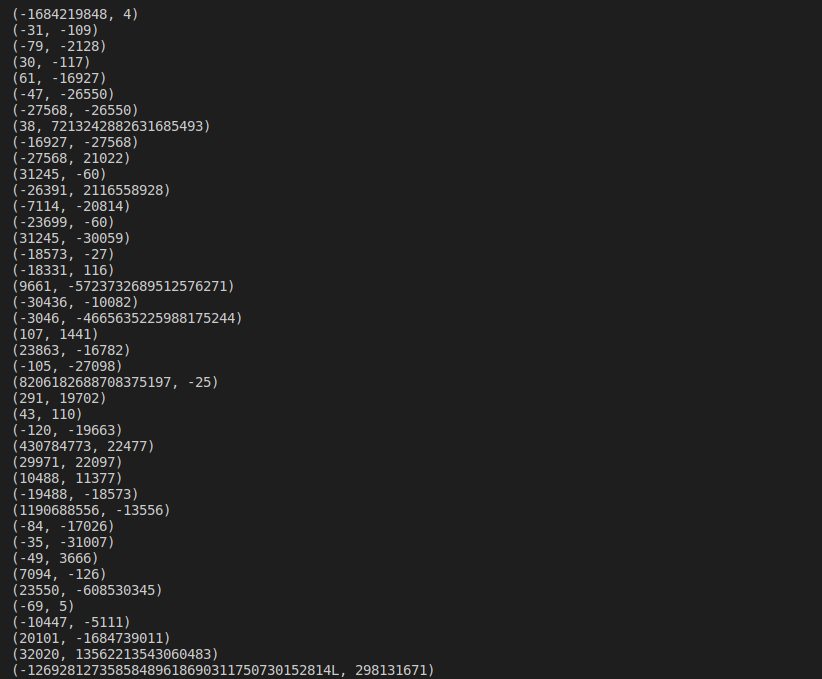
\includegraphics[width=10cm,height=10cm,keepaspectratio]{testing_1.png}
	\caption{A sample of the input generated by strategies.}
	\label{fig 2: strategies' input.}
\end{figure}
And That's basically it to get started with hypothesis, just knowing the correct strategy and the property that's guaranteed in the output of the tested function.
 
\section{{\large Details and Advanced Features}}
This section lists features that are less common in Hypothesis but make life much easier.
Each Feature is followed by a use case.
\subsection{Additional test output}
note()
\subsection{Test statistics}
\subsection{Making Assumptions}
\subsection{Defining strategies}
\subsection{Making random code deterministic}
\subsection{Inferred strategies}



\section{{\large Limitations}}

\section{{\large Case Study}}

\section {{\large Work Load Divison}}

\section {{\large References}}




\end{document}
